\documentclass[10pt,a4paper]{article}
\usepackage[utf8]{inputenc}
\usepackage{amsmath}
\usepackage{gensymb}
\usepackage{amsfonts}
\usepackage{siunitx}
\usepackage[european]{circuitikz}
\usepackage{geometry}
\newgeometry{tmargin=2cm, bmargin=2cm, lmargin=2cm, rmargin=2cm}
\usepackage{amssymb}
\usepackage{multirow}
\usepackage{polski}
\usepackage{graphicx}
\author{\textbf{T. Fąs}}
\title{\textbf{WZMACNIACZ TRANZYSTOROWY}}
\begin{document}
\maketitle

\begin{center}
\textbf{\subsection*{STRESZCZENIE}}
\end{center}
W doświadczeniu badano własności tranzystora, wyznaczano jego punkt pracy oraz własności wzmacniacza o wspólnym emiterze. Otrzymane wartości były zgodne z przewidywaniami.


\begin{center}
\textbf{\subsection*{WSTĘP}}
\end{center}

Tranzystor to element elektroniczny oparty o materiały półprzewodnikowe, który jest zdolny do wzmacniania sygnału. Schemat tranzystora bipolarnego przedstawiono na Rysunku 1. 

\begin{figure}[h!]
\centering
\begin{minipage}{0.5\textwidth}
  \centering
  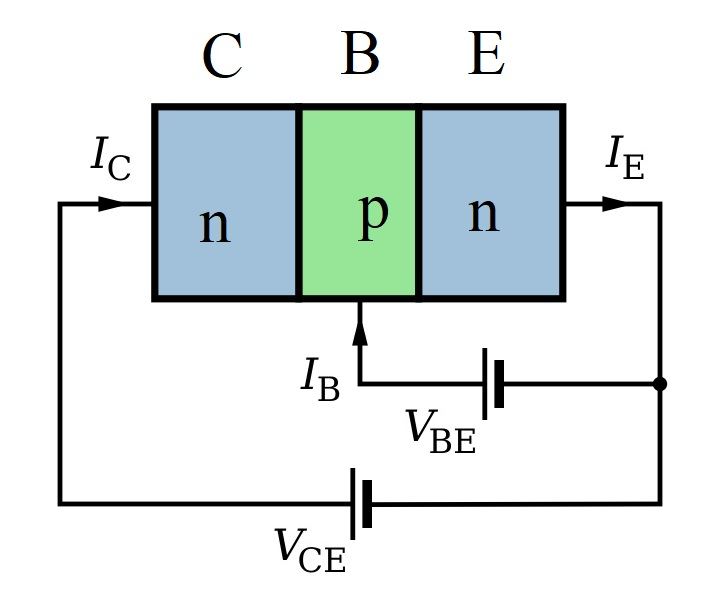
\includegraphics[width=8cm, height=5cm ]{rap21rys3} 
\caption{Schemat tranzystora.}
\end{minipage}%
\begin{minipage}{0.5\textwidth}
  \centering
  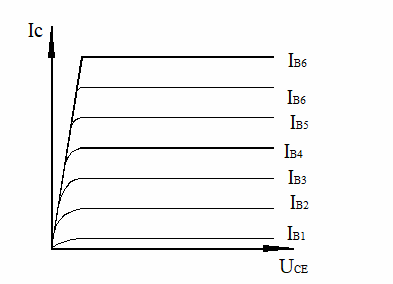
\includegraphics[width=8cm, height=5cm ]{rap21rys4} 
\caption{Zależność $I_{C}$ od $U_{CE}$.}
\end{minipage}
\end{figure}

Zależność między prądem bazy $I_{B}$ a prądem kolektora $I_{C}$ dana jest wzorem:

\begin{equation}
I_{C}=\beta I_{B}.
\end{equation}

Tak więc mały prąd bazy może zostać wielokrotnie wzmocniony, przy czym konieczne jest zastosowanie źródła energii, w tym przypadku w postaci napięcia $U_{CE}$. Przykładowe wzmocnienie prądu bazy w zależności od napięcia zasilającego $U_{CE}$ przedstawiono na Rysunku 2. Jak widać, wzmocnienie to nie jest osiągane natychmiastowo. Ze względu na istnienie takiej zależności wprowadzono pojęcie punktu pracy, dla którego to tranzystor pracuje w optymalnych warunkach. Dla wzmacniacza o wspólnym emiterze, przedstawionego na Rysunku (4), punkt pracy definiuje się jako punkt, dla którego napięcie kolektor-emiter jest połową napięcia zasilającego. Osiąga się to poprzez odpowiedni opornik bocznikowy $R_{B}$.


 Dla wzmacniacza o wspólnym emiterze stosunek napięcia wyjściowego $U_{WY}$ do napięcia wejściowego $U_{WE}$ jest kombinacją odpowiednio przeskalowanych transmitancji filtru kolejno górno- i dolno- przepustowego, czyli zależy od częstości $\omega$ sygnału wejściowego. Odpowiednie równania są następujące:
 
 \begin{equation}
 \left|\dfrac{U_{WY}}{U_{WE}}\right|=\dfrac{k\omega}{\sqrt{\omega^2+\omega_{k1}^2}}
 \end{equation}
 
  \begin{equation}
  \left|\dfrac{U_{WY}}{U_{WE}}\right|=\dfrac{k\omega_{k2}}{\sqrt{\omega^2+\omega_{k2}^2}}
 \end{equation}

Przy czym $k$ jest współczynnikiem wzmocnienia, a $\omega_{k1}$ i $\omega_{k2}$ to wartości częstości, dla których wzmocnienie przyjmuje wartość $k/\sqrt{2}$.

W doświadczeniu wykorzystano układ przedstawiony na Rysunku 3 do zbadania zależności z Równania (1) oraz do wyznaczenia punktu pracy tranzystora, korzystając z zależności:

\begin{equation}
R_{B}=2R_{L}\beta\left(\dfrac{\mathcal{E}-0,65V}{\mathcal{E}}\right).
\end{equation}

Z kolei układ z Rysunku 4 wykorzystano do wyznaczenia wartości $R_{B}$ poprzez manipulację  opornikiem $R_{B1}$ oraz do wyznaczenia zależności napięcia wyjściowego od napięcia wejściowego, jak i zależności współczynnika wzmocnienia od częstości napięcia wejściowego.

\begin{center}
\textbf{\subsection*{UKŁAD DOŚWIADCZALNY}}
\end{center}

\begin{figure}[h!]
\centering
\begin{minipage}{0.5\textwidth}
  \centering
  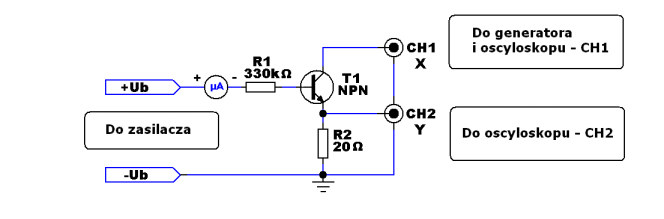
\includegraphics[width=8cm, height=5cm ]{rap21rys1} 
\caption{Schemat pierwszego obwodu \cite{r1}.}
\end{minipage}%
\begin{minipage}{0.5\textwidth}
  \centering
  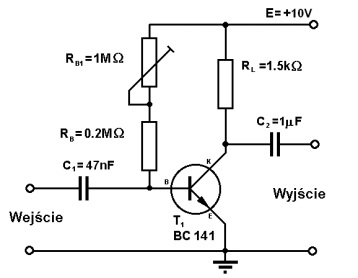
\includegraphics[width=8cm, height=5cm ]{rap21rys2} 
\caption{Schemat drugiego obwodu \cite{r1}.}
\end{minipage}
\end{figure}

W doświadczeniu wykorzystano układy z Rysunku 3 i Rysunku 4, tranzystor bipolarny NPN, miernik uniwersalny, oscyloskop, zasilacz oraz generator sygnałów. W przypadku układu z Rysunku 3 wykorzystano miernik uniwersalny do pomiarów natężenia prądu bazy $I_{B}$, a oscyloskop do pomiarów napięcia na oporniku $R2$. Dzięki temu można było poznać natężenie $I_{C}$ dzieląc otrzymane napięcie przez wartość oporu $R2$. Generatorem prądu bazy był zasilacz prądu stałego. 

W przypadku układu z Rysunku 4 do wejścia podłączono generator sygnałów, a wyjście podłączono do oscyloskopu. Dodatkowo połączono też bezpośrednio generator i oscyloskop. Aby wyznaczyć wartość oporu bocznikowego manipulowano wartością oporu opornika $R_{B1}$ oraz mierzono napięcie na kolektorze miernikiem uniwersalnym. W przypadku pomiarów współczynnika wzmocnienia mierzono napięcie wyjściowe przy pomocy oscyloskopu.

\begin{center}
\textbf{\subsection*{WYNIKI POMIARÓW}}
\end{center}

Wyniki pomiarów zależności prądu kolektora od prądu bazy przedstawiono w Tabeli 1. W tabeli umieszczono też wartość oporu $R2$. Pomiarów dokonywano dla wejściowego sygnału piłokształtnego o amplitudzie 10 V i częstotliwości 100 Hz, a pomiar napięcia zdejmowano w obszarze plateau zależności z Rysunku 2.

\begin{table}[h!]
\centering
\caption{Wyniki pomiarów: prąd bazy i kolektora.}

\begin{tabular}{|c|c|c|c|}
\hline
$I_{B}$ [$\mu$A] & $U_{C}$ [mA] & $I_{B}$ [$\mu$A]   & $U_{C}$ [mA]   \\ \hline
5,965            & 20           & 22,953             & 100            \\ \hline
8,147            & 30           & 25,073             & 110            \\ \hline
10,168           & 40           & 27,319             & 120            \\ \hline
12,249           & 50           & 29,162             & 130            \\ \hline
14,539           & 60           & 31,438             & 140            \\ \hline
16,534           & 70           & 33,467             & 150            \\ \hline
18,741           & 80           & 36,187             & 160            \\ \hline
20,948           & 90           & \multicolumn{2}{c|}{$R2=20$ $\Omega$} \\ \hline
\end{tabular}
\end{table}
 
W Tabeli 2 przedstawiono wartości napięcia wejściowego i wyjściowego dla układu z Rysunku 4 dla sygnału sinusoidalnego o częstości 1 kHz.


\begin{table}[h!]
\centering
\caption{Wyniki pomiarów: wzmocnienie sygnału wyjściowego; stała częstość.}
\begin{tabular}{|c|c|c|c|}
\hline
$U_{WE}$ [mV] & $U_{WY}$ [V] & $U_{WE}$ [mV] & $U_{WY}$ [V] \\ \hline
51,6          & 4,36         & 10            & 0,88         \\ \hline
61,2          & 5,16         & 27            & 2,24         \\ \hline
72            & 6            & 36,6          & 3,08         \\ \hline
82,1          & 6,72         & 46,8          & 3,96         \\ \hline
92,2          & 7,5          & 56,8          & 4,76         \\ \hline
102           & 8,21         & 66            & 5,56         \\ \hline
112           & 8,63         & 76,4          & 6,32         \\ \hline
122           & 8,91         & 87,1          & 7,16         \\ \hline
42,2          & 3,52         & 96,3          & 7,84         \\ \hline
31,3          & 2,66         & 107           & 8,53         \\ \hline
21,8          & 1,8          & 117           & 8,83         \\ \hline
\end{tabular}
\end{table}

Tabela 3 przedstawia wartości napięcia wyjściowego w zależności od częstości sygnału wejściowego. 

\begin{table}[h!]
\centering
\caption{Wyniki pomiarów: wzmocnienie sygnału wyjściowego; zmienna częstość.}
\label{my-label}
\begin{tabular}{|c|c|c|c|c|c|}
\hline
$U_{WE}$ [mV] & $U_{WY}$ [V] & $f=\omega/2\pi$ [Hz] & $U_{WE}$ [mV] & $U_{WY}$ [V] & $f=\omega/2\pi$ [Hz] \\ \hline
53,2          & 87           & 10                   & 50,4          & 7680         & 8000                 \\ \hline
52,8          & 133          & 15                   & 50            & 7680         & 10000                \\ \hline
52,8          & 181          & 30                   & 50            & 7730         & 20000                \\ \hline
53,2          & 284          & 50                   & 50            & 7680         & 30000                \\ \hline
53,6          & 440          & 80                   & 50            & 7630         & 50000                \\ \hline
52,4          & 541          & 100                  & 48,8          & 7580         & 80000                \\ \hline
52,4          & 789          & 150                  & 48,8          & 7480         & 100000               \\ \hline
52            & 1530         & 300                  & 48,4          & 7190         & 200000               \\ \hline
52            & 3680         & 800                  & 46,8          & 6840         & 300000               \\ \hline
52            & 4360         & 1000                 & 44,4          & 6100         & 500000               \\ \hline
51,2          & 6280         & 2000                 & 40,4          & 5110         & 800000               \\ \hline
51,6          & 7040         & 3000                 & 38            & 4460         & 1000000              \\ \hline
50,8          & 7550         & 5000                 & \multicolumn{3}{c|}{}                               \\ \hline
\end{tabular}
\end{table}

Manipulując wartością oporu $R_{B1}$ udało się osiągnąć punkt pracy dla wartości oporu bocznikowego $R_{B}=630,5$ k$\Omega$.

\begin{center}
\textbf{\subsection*{ANALIZA DANYCH}}
\end{center}

Korzystając z danych z Tabeli 1 wykonano wykres zależności prądu kolektora od prądu bazy. Wykres przedstawiono na Rysunku 5. Do wykresu dopasowano prostą postaci $ax+b$, gdzie $a=\beta$, a $b$ jest przesunięciem wynikłym z przyjętych przybliżeń. Przyjęto niepewność 2\% wartości $I_{C}$.


\begin{figure}[h!]
\centering
\begin{minipage}{0.5\textwidth}
  \centering
  \advance\leftskip-0.5cm
 \centerline{ 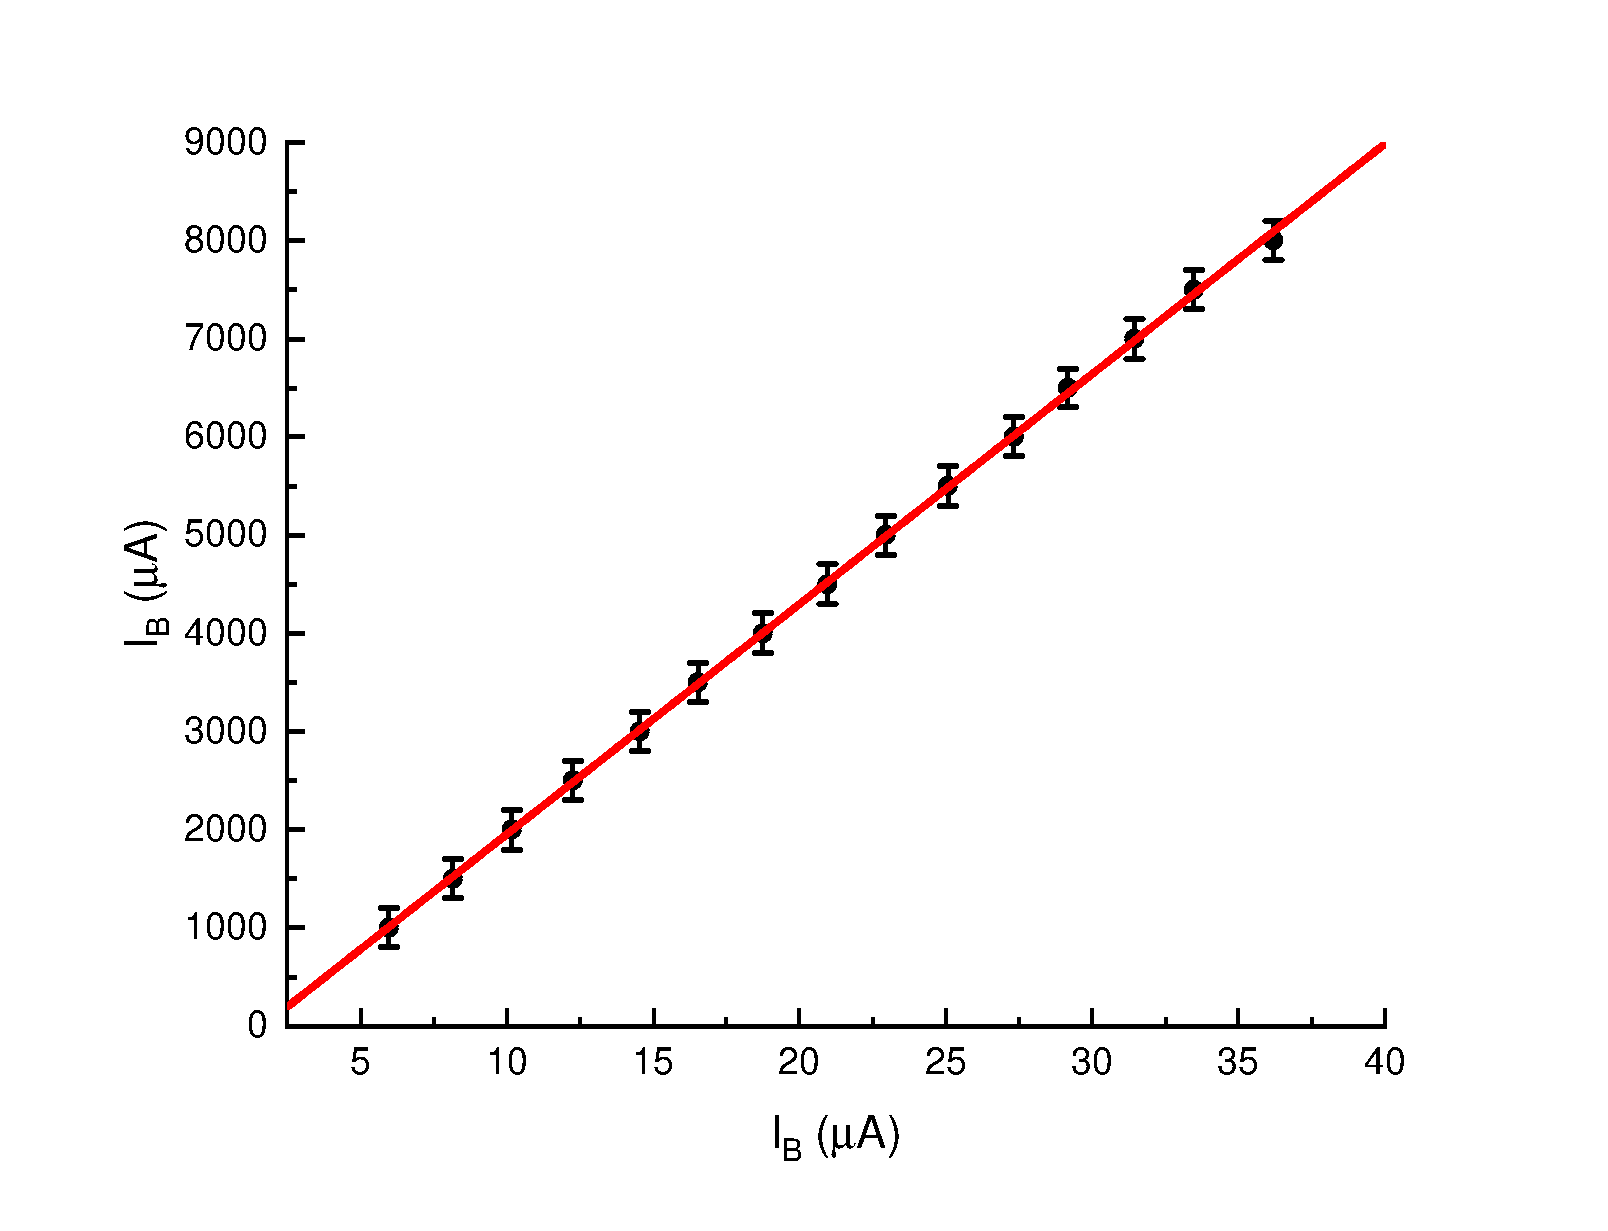
\includegraphics[width=12cm]{rap21rys4.pdf} }
\caption{Zależność $I_{C}(I_{B})$.}
\end{minipage}%
\begin{minipage}{0.5\textwidth}
  \centering
   \advance\leftskip-0.5cm
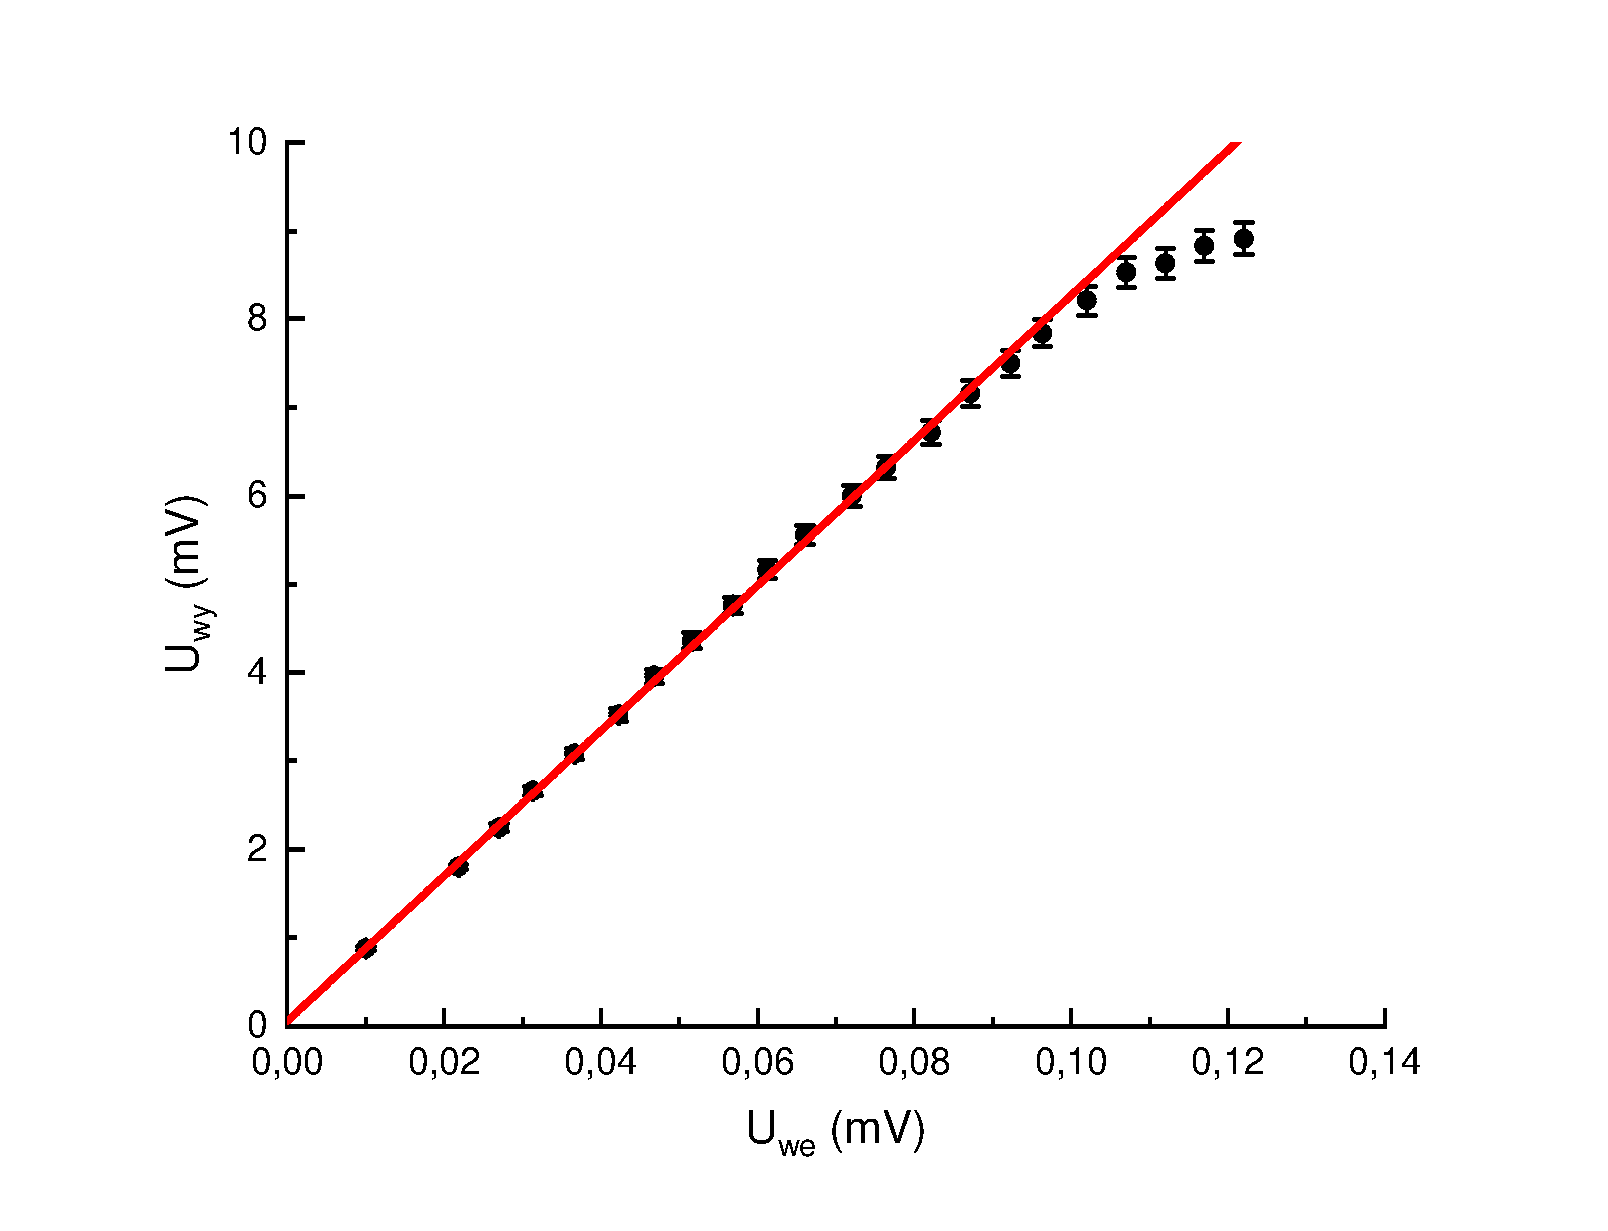
\includegraphics[width=12cm]{rap21rys5.pdf} 
\caption{Zależność $U_{WY}(U_{WE})$.}
\end{minipage}
\end{figure}


Otrzymano wartości: $\beta=234,4\pm1,0$ i $b=-390\pm23$ $\mu$A.

Korzystając z tej wartości $\beta$ oraz z wartości $R_{L}$=1,5 k$\Omega$ i $\mathcal{E}=10$ V otrzymujemy $R_{B}=657,52$ k$\Omega$. Różnica wartości zmierzonej i obliczonej wynosi 27 k$\Omega$, czyli około 4\% wartości zmierzonej. Jest to różnica na tyle mała, że można uznać te wartości za zgodne ze sobą.


Na Rysunku 6 przedstawiono wykres dla wartości z Tabeli 2 wraz z krzywą najlepszego dopasowania postaci $ax+b$. Przyjęto niepewność 2\% wartości $U_{WY}$. Otrzymane wartości to $a=82,14\pm0,51$ i $b=0,058\pm0,014$ V. Krzywa ta jest bardzo dobrze dopasowana w obszarze liniowego wzmocnienia.




Rysunek 7 przedstawia dane z Tabeli 3 w skali logarytmicznej wraz z odpowiednio przeskalowanymi o czynnik $2\pi$ wartościami częstości. Do tych danych dopasowano zależności z Równania (2) i Równania (3), przy czym punktem granicznym była wartość 30 kHz. Tak jak wcześniej przyjęto błąd 2\%. Otrzymano następujące parametry dopasowania: $k_{1}=152,1\pm8,4$, $\omega_{k1}=8600\pm660$ 1/s, $k_{2}=152,6\pm0,9$ i $\omega_{k2}=7400000\pm240000$ 1/s. Parametry $k$ są ze sobą zgodne na mocy testu 3$\sigma$.

\begin{figure}[h!]
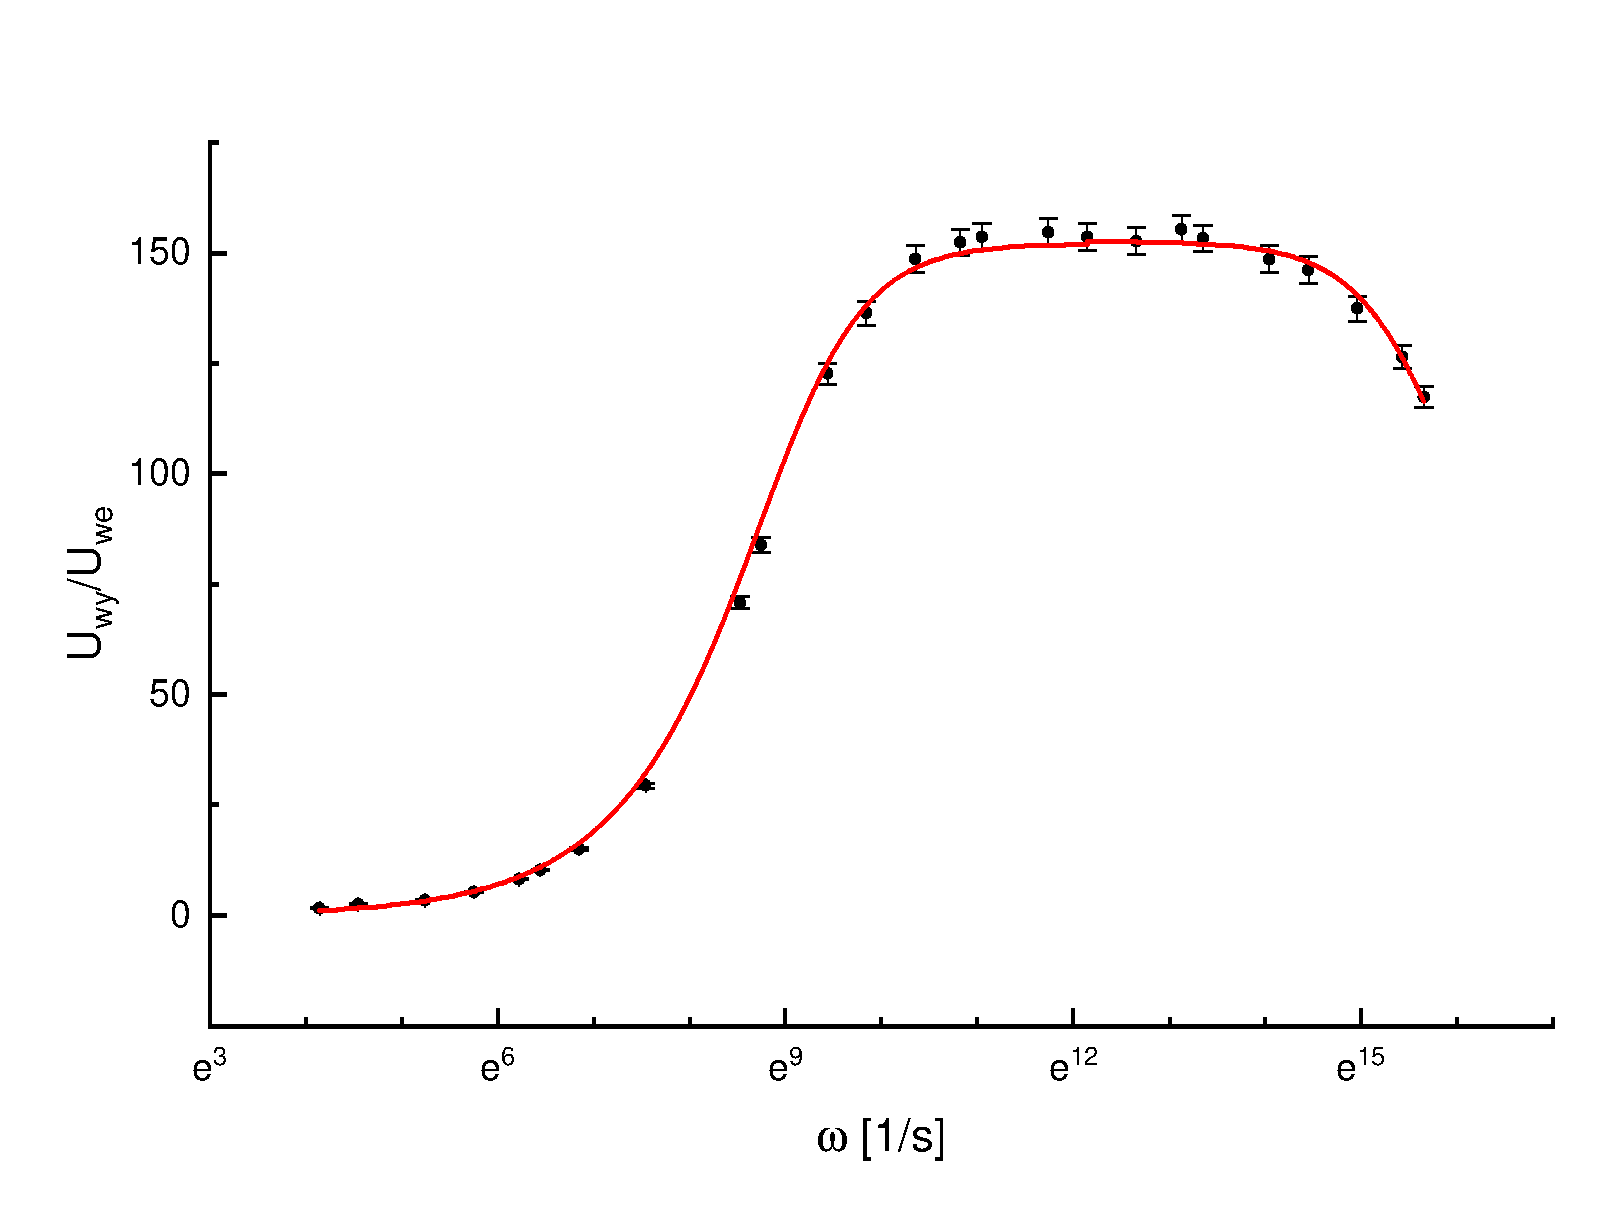
\includegraphics[width=13cm]{rap21rys6.pdf} 
\centering
\caption{Zależność $U_{WY}(\omega)$.}
\end{figure}


Jeśli założyć, że na wejściu wzmacniacza istnieje filtr górnoprzepustowy o oporze $R$, pojemności $C_{1}=47$ nF i częstości krytycznej $\omega_{k1}$, to opór wejściowy tego wzmacniacza wynosi $R=0,28$ $\Omega$.




\begin{center}
\textbf{\subsection*{DYSKUSJA WYNIKÓW I WNIOSKI}}
\end{center} 

Tranzystor oraz wzmacniacz zachowywał się zgodnie z oczekiwaniami i do wszystkich zależności udało się dopasować krzywe teoretyczne. Otrzymane wartości współczynników wzmocnienia były właściwego rzędu wielkości, a wartości oporu bocznikowego, otrzymane dwoma różnymi metodami, były ze sobą zgodne. W skrócie: pomiary zostały zakończone sukcesem.



\begin{center}
\begin{thebibliography}{9}

\bibitem{r1}
 Praca zbiorowa,
 \emph{Instrukcja do ćwiczenia "Wzmacniacz tranzystorowy"},
 FUW, Warszawa, 2016.
 
 
 
 \end{thebibliography}

\end{center}


\end{document}